\documentclass{sigchi}

% Use this command to override the default ACM copyright statement
% (e.g. for preprints).  Consult the conference website for the
% camera-ready copyright statement.


%% EXAMPLE BEGIN -- HOW TO OVERRIDE THE DEFAULT COPYRIGHT STRIP -- (July 22, 2013 - Paul Baumann)
% \toappear{Permission to make digital or hard copies of all or part of this work for personal or classroom use is      granted without fee provided that copies are not made or distributed for profit or commercial advantage and that copies bear this notice and the full citation on the first page. Copyrights for components of this work owned by others than ACM must be honored. Abstracting with credit is permitted. To copy otherwise, or republish, to post on servers or to redistribute to lists, requires prior specific permission and/or a fee. Request permissions from permissions@acm.org. \\
% {\emph{CHI'14}}, April 26--May 1, 2014, Toronto, Canada. \\
% Copyright \copyright~2014 ACM ISBN/14/04...\$15.00. \\
% DOI string from ACM form confirmation}
%% EXAMPLE END -- HOW TO OVERRIDE THE DEFAULT COPYRIGHT STRIP -- (July 22, 2013 - Paul Baumann)


% Arabic page numbers for submission.  Remove this line to eliminate
% page numbers for the camera ready copy 

%\pagenumbering{arabic}

% Load basic packages
\usepackage{balance}  % to better equalize the last page
\usepackage{graphics} % for EPS, load graphicx instead 
%\usepackage[T1]{fontenc}
\usepackage{txfonts}
\usepackage{times}    % comment if you want LaTeX's default font
\usepackage[pdftex]{hyperref}
% \usepackage{url}      % llt: nicely formatted URLs
\usepackage{color}
\usepackage{textcomp}
\usepackage{booktabs}
\usepackage{ccicons}
\usepackage{todonotes}
\usepackage{subfigure}
\usepackage{multirow}

% llt: Define a global style for URLs, rather that the default one
\makeatletter
\def\url@leostyle{%
  \@ifundefined{selectfont}{\def\UrlFont{\sf}}{\def\UrlFont{\small\bf\ttfamily}}}
\makeatother
\urlstyle{leo}

% To make various LaTeX processors do the right thing with page size.
\def\pprw{8.5in}
\def\pprh{11in}
\special{papersize=\pprw,\pprh}
\setlength{\paperwidth}{\pprw}
\setlength{\paperheight}{\pprh}
\setlength{\pdfpagewidth}{\pprw}
\setlength{\pdfpageheight}{\pprh}

% Make sure hyperref comes last of your loaded packages, to give it a
% fighting chance of not being over-written, since its job is to
% redefine many LaTeX commands.
\definecolor{linkColor}{RGB}{6,125,233}
\hypersetup{%
  pdftitle={SIGCHI Conference Proceedings Format},
  pdfauthor={LaTeX},
  pdfkeywords={SIGCHI, proceedings, archival format},
  bookmarksnumbered,
  pdfstartview={FitH},
  colorlinks,
  citecolor=black,
  filecolor=black,
  linkcolor=black,
  urlcolor=linkColor,
  breaklinks=true,
}

% create a shortcut to typeset table headings
% \newcommand\tabhead[1]{\small\textbf{#1}}

% End of preamble. Here it comes the document.
\begin{document}
\author{
  Yvonne Chen\\
  \texttt{evechen@uw.edu}
  \and
  Eleanor O'Rourke\\
  \texttt{eorourke@cs.washington.edu}
}
\title{Visualizing Student Problem-Solving Data}


\maketitle

\begin{abstract}
Abstract goes here
\end{abstract}


%\keywords{Technology in the classroom; tablets for education; adaptive learning environments.}

%\category{H.5.0.}{Information Interfaces and Presentation}{General}

\section{Introduction}
An explanation of the problem and the motivation for solving it.

\section{Related Work}
A large body of research has explored methods of integrating technology into in-person classrooms and using technology to deliver education online. We review this research focusing on technology-delivered curriculums, systems that expose student data for teachers, and adaptive learning environments.

\subsection{Exposing Student Data for Teachers}
Education research shows that teacher behavior has a strong impact on student achievement \cite{Hill2005, Wentzel2002, Reeve2004, Wright1997}, and that teachers can benefit from the availability of real-time student data \cite{Balaam2010, Koile2006, Lazar2007}. For example, Koile found that when an instructor was given access to student problem solutions through tablet-based technology in real-time, the instructor devoted 75\% of class time responding to student misunderstandings \cite{Koile2006}. With access to real-time data, research suggests that instructors can intervene during a lesson when students are confused \cite{Hickey2014}, alter the pace or content of instruction based on student engagement \cite{Balaam2010}, immediately identify and assist students who are struggling \cite{Lazar2007}, and choose topics of focus based on aggregates of student responses \cite{Koile2006}. 

A number of technologies have been developed for exposing student data for teachers. One technology that is often used in lecture-based classes is the ``student response system'' or ``clicker,'' which is used to poll students on multiple-choice questions during class \cite{Dangel08, Lazar2007}. A similar application designed for small classes is Plickers \cite{Plickers}. With the Plickers smartphone app, the teacher can scan the classroom while students hold up QR codes identifying a multiple-choice answer \cite{Plickers}. Researchers have also explored methods of providing instructors with access to student data outside of instruction time to monitor longer term academic progress \cite{Zhang2015, Arnold2012}. Kim et.\ al.\ developed a system for compiling student responses to MOOC exercise problems, which teachers reported were useful for capturing student thought processes, identifying misconceptions, and engaging students with content \cite{Kim2015}.

In this work, we explore methods of exposing rich problem-solving data to elementary school teachers in real-time. Through a longitudinal study, we explore how teacher behavior is impacted by exposing information about student misconnects and progress through curriculum material.

Whether viewed in real time or after the fact, teachers benefit from the availability of student data. Accessed in real time, student data affords immediate intervention. In a study by Koile, students used Tablet PCs to complete exercise problems during class time. The instructor could access their answers right away on her own device. Based on the students' answers, the instructor devoted 75\% of course time responding to misunderstandings of course material, and would delay or hasten presentation of new material as appropriate \cite{Koile2006}. With real time student data, instructors can intervene during a lesson when students are confused \cite{Hickey2014}, alter the pace or content of instruction based on student engagement \cite{Balaam2010}, immediately identify and assist students who are struggling \cite{Lazar2007}, and choose topics of focus based on aggregates of student responses \cite{Koile2006}.

When timely intervention is less critical, instructors can view data outside of instruction time to
monitor longer term academic progress \cite{Zhang2015, Arnold2012}. Kim et al developed an online system for teachers to author video lectures containing integrated multimedia exercises. The system compiled student responses as they completed exercises, and teachers reported that they were useful for ``capturing students\' thought processes, identifying misconceptions, and engaging students with content'' \cite{Kim2015}. Even basic classroom response systems, which poll students to choose one out of a set of pre-defined responses, give teachers a quick aggregate overview of student understanding \cite{Lazar2007}.

While research shows that student data can help teachers understand misconceptions and how they spend class time, very little is known about how to visualize student data to most effectively communicate with teachers. We have not encountered any papers that study the design of visualizations of student data. Enlearn has implemented two different methods of visualizing student data in real-time for teachers, however, both of their designs have had usability and readability problems when tested in classrooms. This shows how challenging it is to create effective visualizations for communicating student data in real-time. Enlearn's first design, shown in Figure 1a, displays a table view of student problem solving pace and correctness. While this visualization provides information about the progress of individual students, it communicates nothing about the specific concepts that students are struggling with. Enlearn's second design, shown in Figure 1b, displays a graph view of student problem solving that is organized by concept. While this displays information about the concepts that students are struggling with, there is no way for teachers to see which individuals are struggling. Most importantly, neither visualization provides teachers with actionable suggestions about how to assist students who are struggling. Prior work shows the utility of communicating student data for instructors, and Enlearn?s experiences with their current visualizations shows the challenge of designing effective means of communicating data, especially in real time for busy teachers. This motivates our desire to improve and strengthen the data visualization for the Enlearn software.

\section{Enlearn}
For this project, we partnered with Enlearn, a non-profit company founded to develop tablet-based adaptive problem-solving software for K-12 classrooms. In our visualizations, we display real data from Enlearn students.

Enlearn evaluated two visualizations with teachers this spring. One displays student data in a table view, but provides no concept-level information. The other displays a concept graph, but provides no data at the level of individual students.

Enlearn found that neither visualization was effective in the classroom, in large part because the information provided did not match teacher needs. Another challenge is that teachers are extremely busy during class time and need visualizations that are both easily glanceable and that provide actionable information.




\section{Methods}
To address the challenge of designing effective techniques for visualizing student problem-solving data for teachers, we first characterize the problem, then discuss our data abstractions, present our visual encodings for conveying the data, and describe our implementation.


\subsection{Problem Characterization}
The initial goal of this research was to understand the format of the problem-solving data collected by the Enlearn software and accurately characterize the tasks that teachers want to accomplish using this data. The challenges that Enlearn faced with their initial visualization designs shows the importance of understanding user needs; Enlearn's visualizations failed in large part because they did not effectively support teacher tasks. While we did not directly meet with teachers, we worked closely with Enlearn staff to understand the feedback they received in response to their initial visualizations. Here we first describe the structure of the problem-solving data collected by Enlearn, and then describe teacher tasks. We provide a set of design guidelines for our visualizations based on this problem characterization.

\subsubsection{Enlearn Data Structure}
In Enlearn classrooms, each student solves problems on a personal tablet. Enlearn logs the following problem-solving information to a database: the id of the student, the id of the problem, the id of the associated problem set, and whether or not the student answered the problem correctly. The Enlearn adaptive curriculum is designed as an extension of the JUMP Math curriculum \cite{JUMPMath}. In JUMP Math, students solve a linear progression of Exercise and Workbook problems. In Enlearn's adaptive version of the curriculum, students practice each type of Exercise or Workbook problem until they have mastered the concept covered by that problem. As a result, students may work on multiple practice problems of the type ``Exercise Problem 3'' before moving on to the next problem type. Enlearn refers to each problem type as a \emph{problem set}, but we use the term \emph{concept} in this paper since it better matches how teachers refer to the groups of problems.

\subsubsection{Teacher Tasks}
Through our discussions with Enlearn staff, we learned that there are two primary tasks that teachers want to accomplish using student problem-solving data during class. First, teachers want to determine which students need individual assistance and what specific concepts they are struggling with at any given moment. Ideally, teachers would also be able to see if multiple students are struggling with the same concept at the same time so that they can pull the students aside to work with them as a group. Second, teachers want to determine how each student is performing overall during the current lesson. If many students are struggling with the content, the teacher may chose to re-teach parts of the lesson.

While Enlearn's initial visualizations tried to target these tasks, they did not provide adequate information for teachers to be able to quickly determine which students were struggling the most and what concepts they were currently working on. The overwhelming feedback that Enlearn was given by teachers after their trial was that the real-time visualizations need to provide information that is glanceable and immediately actionable. During class, teachers are busy adapting lessons, responding to students, and managing organizational challenges. They do not have time to explore a complex visualization of student data. Instead, they need a simple view that provides them with the exact information they need to accomplish in-class tasks such as assisting students and adapting their teaching strategy.

\subsubsection{Design Guidelines}
From our characterization of the structure of Enlearn's problem-solving data and the tasks that teachers need to accomplish using that data, we developed the following design guidelines for our visualizations:

\begin{itemize} \itemsep5pt \parskip0pt \parsep0pt
  \item Visualizations must provide actionable information that clearly displays student performance on practice problems.
  \item Visualizations must show data for individual students so that teachers can easily intervene when needed.
  \item Visualizations must display concept-level data so that teachers can assess student understanding of each concept.
\end{itemize}

We use these guidelines throughout the remainder of our work focus our data abstraction and visual encoding designs.


\subsection{Data Abstractions}





\subsection{Visual Encodings}

\subsubsection{Simulating Real-Time Data}
Our visualizations are designed to display real-time student data; however, we do not have a constant stream of data to display. To simulate real-time problem solving, we use data collected from students last fall. We display a timeline that can be played and brushed, allowing both us and Enlearn staff to quickly see what the visualizations would look like in various real-time scenarios. 

\subsubsection{Concept View}
The concept visualization is designed to help teachers determine which students need help in the present moment. Students are grouped by the concept that they are currently working on so that it is easy for the teacher to know what concept to target. The background color of each student bar indicates how well the student is performing on that concept. This view gives teachers a glanceable display that can help them rapidly determine which student to assist.

\subsubsection{Aggregated View}
The aggregate visualization is designed to give teachers a high-level overview of how each student has performed over the course of the lesson. This view displays all problem-solving information for each student across multiple concepts. The background is colored to show the student's aggregate performance.  If the teacher wants to see concept-level information for a given student, she can click on that student to see the individual visualization shown to the right above.

\subsubsection{Visualization Options}

{\bf Tablet Graphic}\\
We added a tablet graphic as a mockup for intended use of our visualization. The tablet's display area is restricted, but users can scroll within the tablet screen to navigate. To prevent confusion with multiple sets of scrollbars, we designed our visualization to fit on a 13" MacBook Pro screen. The horizontal view and aggregate views are shown in a vertical and horizontal tablet layout, respectively. The concept view tends to grow vertically faster than in grows horizontally, since it only displays problem information for the student's current concept, whereas the aggregate view tends to grow horizontally much faster than it grows vertically, because there is a fixed number of rows based on the number of students in the class.

{\bf Correctness Colors}\\
The default 7-step gradient of colors to represent student problem correctness ranges from a muted orange to a muted green, with yellow as the midpoint - these colors were selected from ColorBrewer2.org, a site created to help designers select easily differentiable color schemes. We chose an orange-green spectrum because red and green are very common encodings for correctness in the educational field - however, we do realize that some users of our tool may be color-blind, so we also include an option to switch to an orange-blue color gradient.

{\bf Button Layout}\\
To provide context to our visualization, the right side of our visualization contains information on the currently selected view, as well as the buttons for various interaction options: switching the view, switching the class session, and switching colors. These buttons are displayed inline with brief descriptions of their purpose.

{\bf Timeline}\\
We display lines on the timeline where problem-solving actions occurred. These visual information scent cues \cite{Willet2007} help to familiarize the viewer with the data set. While we designed this feature for our benefit as designers, it may be valuable when used by teachers to play back their lessons.

{\bf Animation}\\
We use animation to signify changes. When the user clicks the button to switch views, the tablet and information box about the current view fade out, and then the new view fades in. In the concept view, student movement to a new concept is shown by a fade out-fade in transition, leaving a small gap amongst the students in their previous concept to highlight the student's prior location. To prevent viewers from becoming overwhelmed by too much visual movement, check and cross marks that signify problem correctness simply pop into existence.

{\bf Data Choices}\\
Our system provides a selection of 5 datasets that the user can switch between freely. The datasets all come from classes taught by a single teacher in a South Seattle school. We envision a teacher using our tool to replay and compare the progress of different class periods, or the same class period over different lessons. 

\subsection{Implementation}
Enlearn's current visualizations are created using the D3.js visualization library. Hence, we also use D3.js, not only to be compatible within Enlearn's existing workflow, but also to prepare a foundation for a future web-based tool so that teachers will not be dependent on the Enlearn tablet software and can view student data from any computer.


\section{Results \& Discussion}
%The visualizations your system produces and data to help evaluate your approach. For example you may include running times, or the time users typically spend generating a visualization using your system.

%What has the audience learned from your work? What new insights or practices has your system enabled? A full blown user study is not expected, but informal observations of use that help evaluate your system are encouraged.
Our final product is a visualization that integrates our concept view and aggregate views, playing back student progress over a math lesson via a timeline slider that supports brushing. Prior work displays student data at an assignment level, which does not afford immediate intervention in the classroom (may be a wild claim, must confirm). Our system simulates real-time, problem level visualizations that teachers can use to track student problem-solving progress. Through the concept view, teachers can immediately see which students need assistance and what to assist them with, and through the aggregate view, teachers can monitor longer term student progress over the course of a lesson. 

On a more general level, our work is not limited to playing back data gathered from Enlearn math tablets. Any data set with information about problem time completion, problem correctness and problem concept grouping could be visualized using our tool.

Overall, attendees of the CSE 512 project poster session reacted positively, commenting that our system was visually clean and easy to understand. One viewer mentioned that he taught middle school students and would find our visualization useful for tracking their progress. %Nell, can confirm? I think it was Kevin who said it

%Image dump can go here
\begin{figure}[t]
\centering
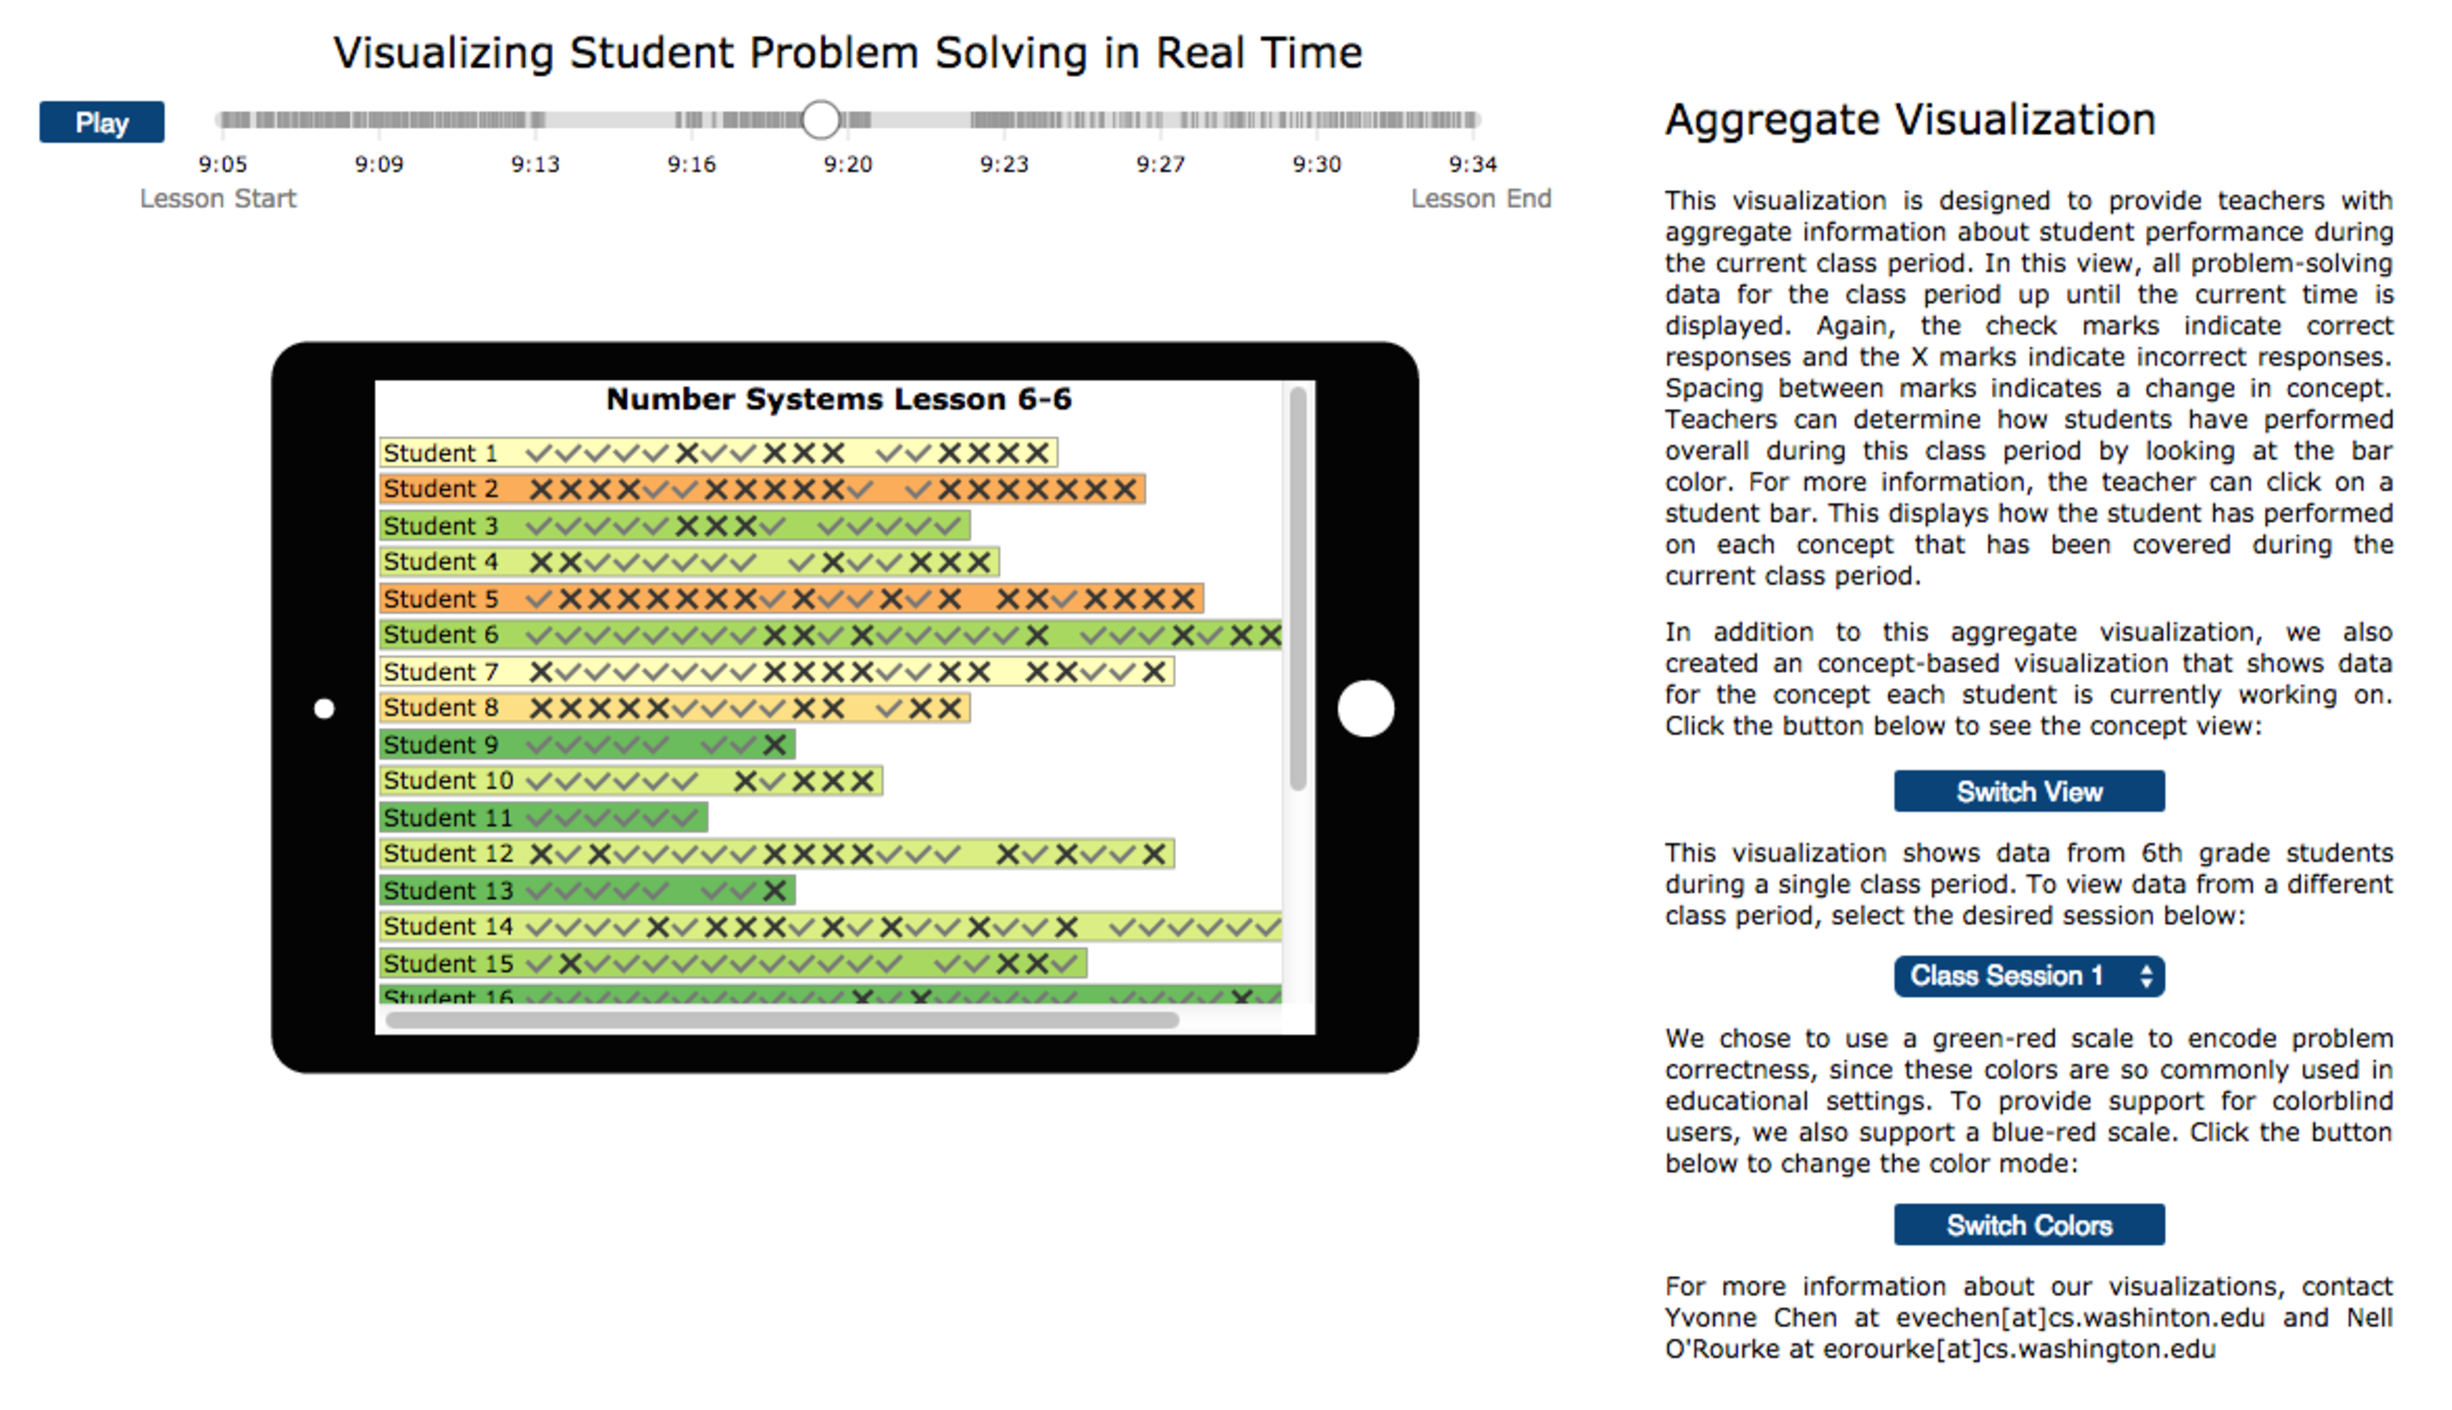
\includegraphics[width=65mm]{images/results1.pdf}
\caption{Caption here}
\label{fig:Results1}
\end{figure}

\section{Future Work}
%A description of how your system could be extended or refined.
As described above, the visual information scent cues overlaid on our timeline slider help inform viewers of gaps where students were not completing tablet problems. The teacher version of Enlearn's software collects data on teacher actions, such as sending a pause signal to freeze all student tablets to get their attention, or switching between lessons. Such information could be overlaid with the timeline slider as insight to teachers. For example, this feature could show that during a time when the teacher is talking, some problem solving activity is still present. This means some students  are off task and using their tablets instead of paying attention to their teacher. However, there is currently no feature to tell which student is associated with which tick marks. Calling out a student's associated tick marks when their name is clicked in the aggregate view would help teachers to monitor an individual student's activity patterns.

Multiple visitors to the poster session that our aggregate view was not as easily glanceable as the concept view. They all independently suggested that information about each student's progress over a single concept could be collapsed into a single representative glyph, such as a shape colored to represent correctness. This way, all students' data could be displayed in a matrix, with pertinent information readily visible at a glance and detailed information accessible by tapping on the student's name. 

Another comment received during the poster session was that our animation transitions could be clearer to help teachers track the movement of students between concepts.

Although the above suggestions have potential to improve our work, an important next step is to evaluate our system with actual teachers. Enlearn has a preexisting relationship with Seattle school teachers, with whom they have collected tablet data over multiple trials. Since Enlearn's current visualizations are also created in D3.js, we can port our system into their software, to be evaluated in future classroom trials. Suggestions from the target audience are invaluable to substantial improvements to our work.

\section{Conclusion}
Our work makes contributions at multiple levels of Munzner?s nested model for visualization design: a characterization of the data visualization needs of classroom teachers, a data abstraction for representing student data grouped by concept, and two new visual encodings for displaying student problem-solving data both streamed in real time and played back after the fact. Our system empowers teachers to easily identify students for real-time assistance, track lesson-level metrics and monitor student progress over multiple lessons.

%\begin{figure*}[t]
%\centering
%\subfigure[]{\label{fig:TeacherLesson}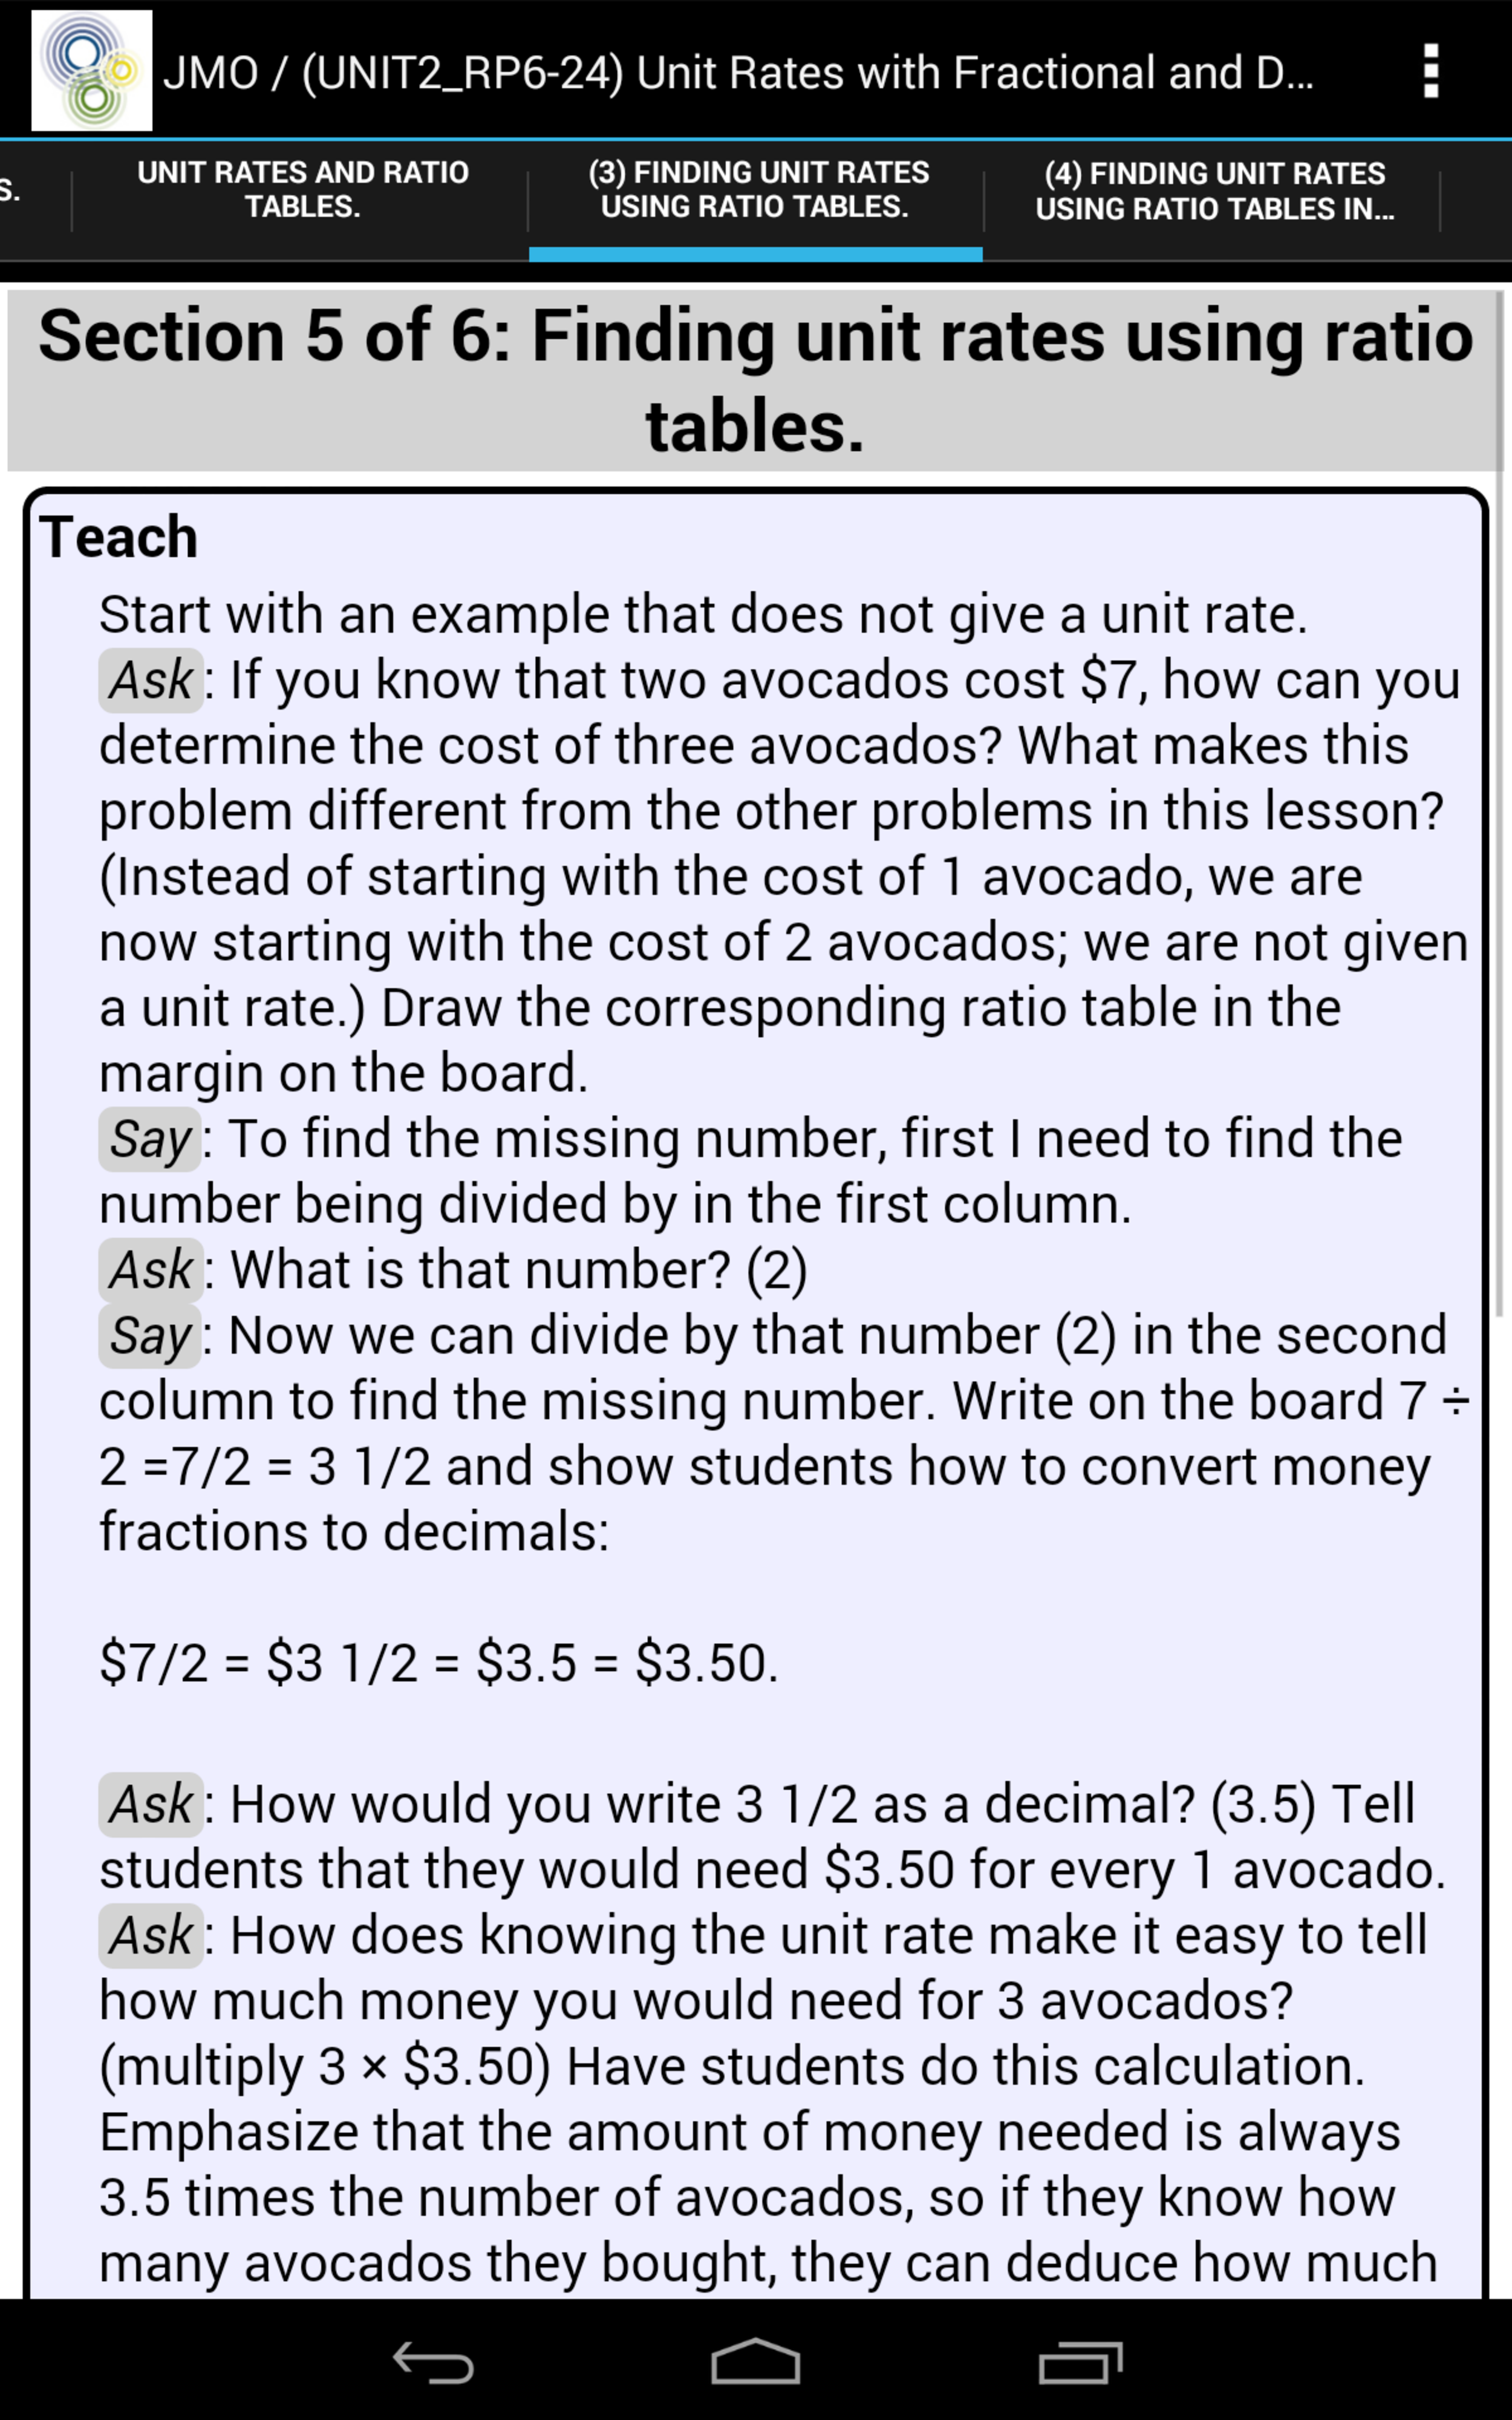
\includegraphics[width=40mm]{images/TeacherLesson.pdf}} \hspace{1em}%
%\subfigure[]{\label{fig:TeacherStartProbems}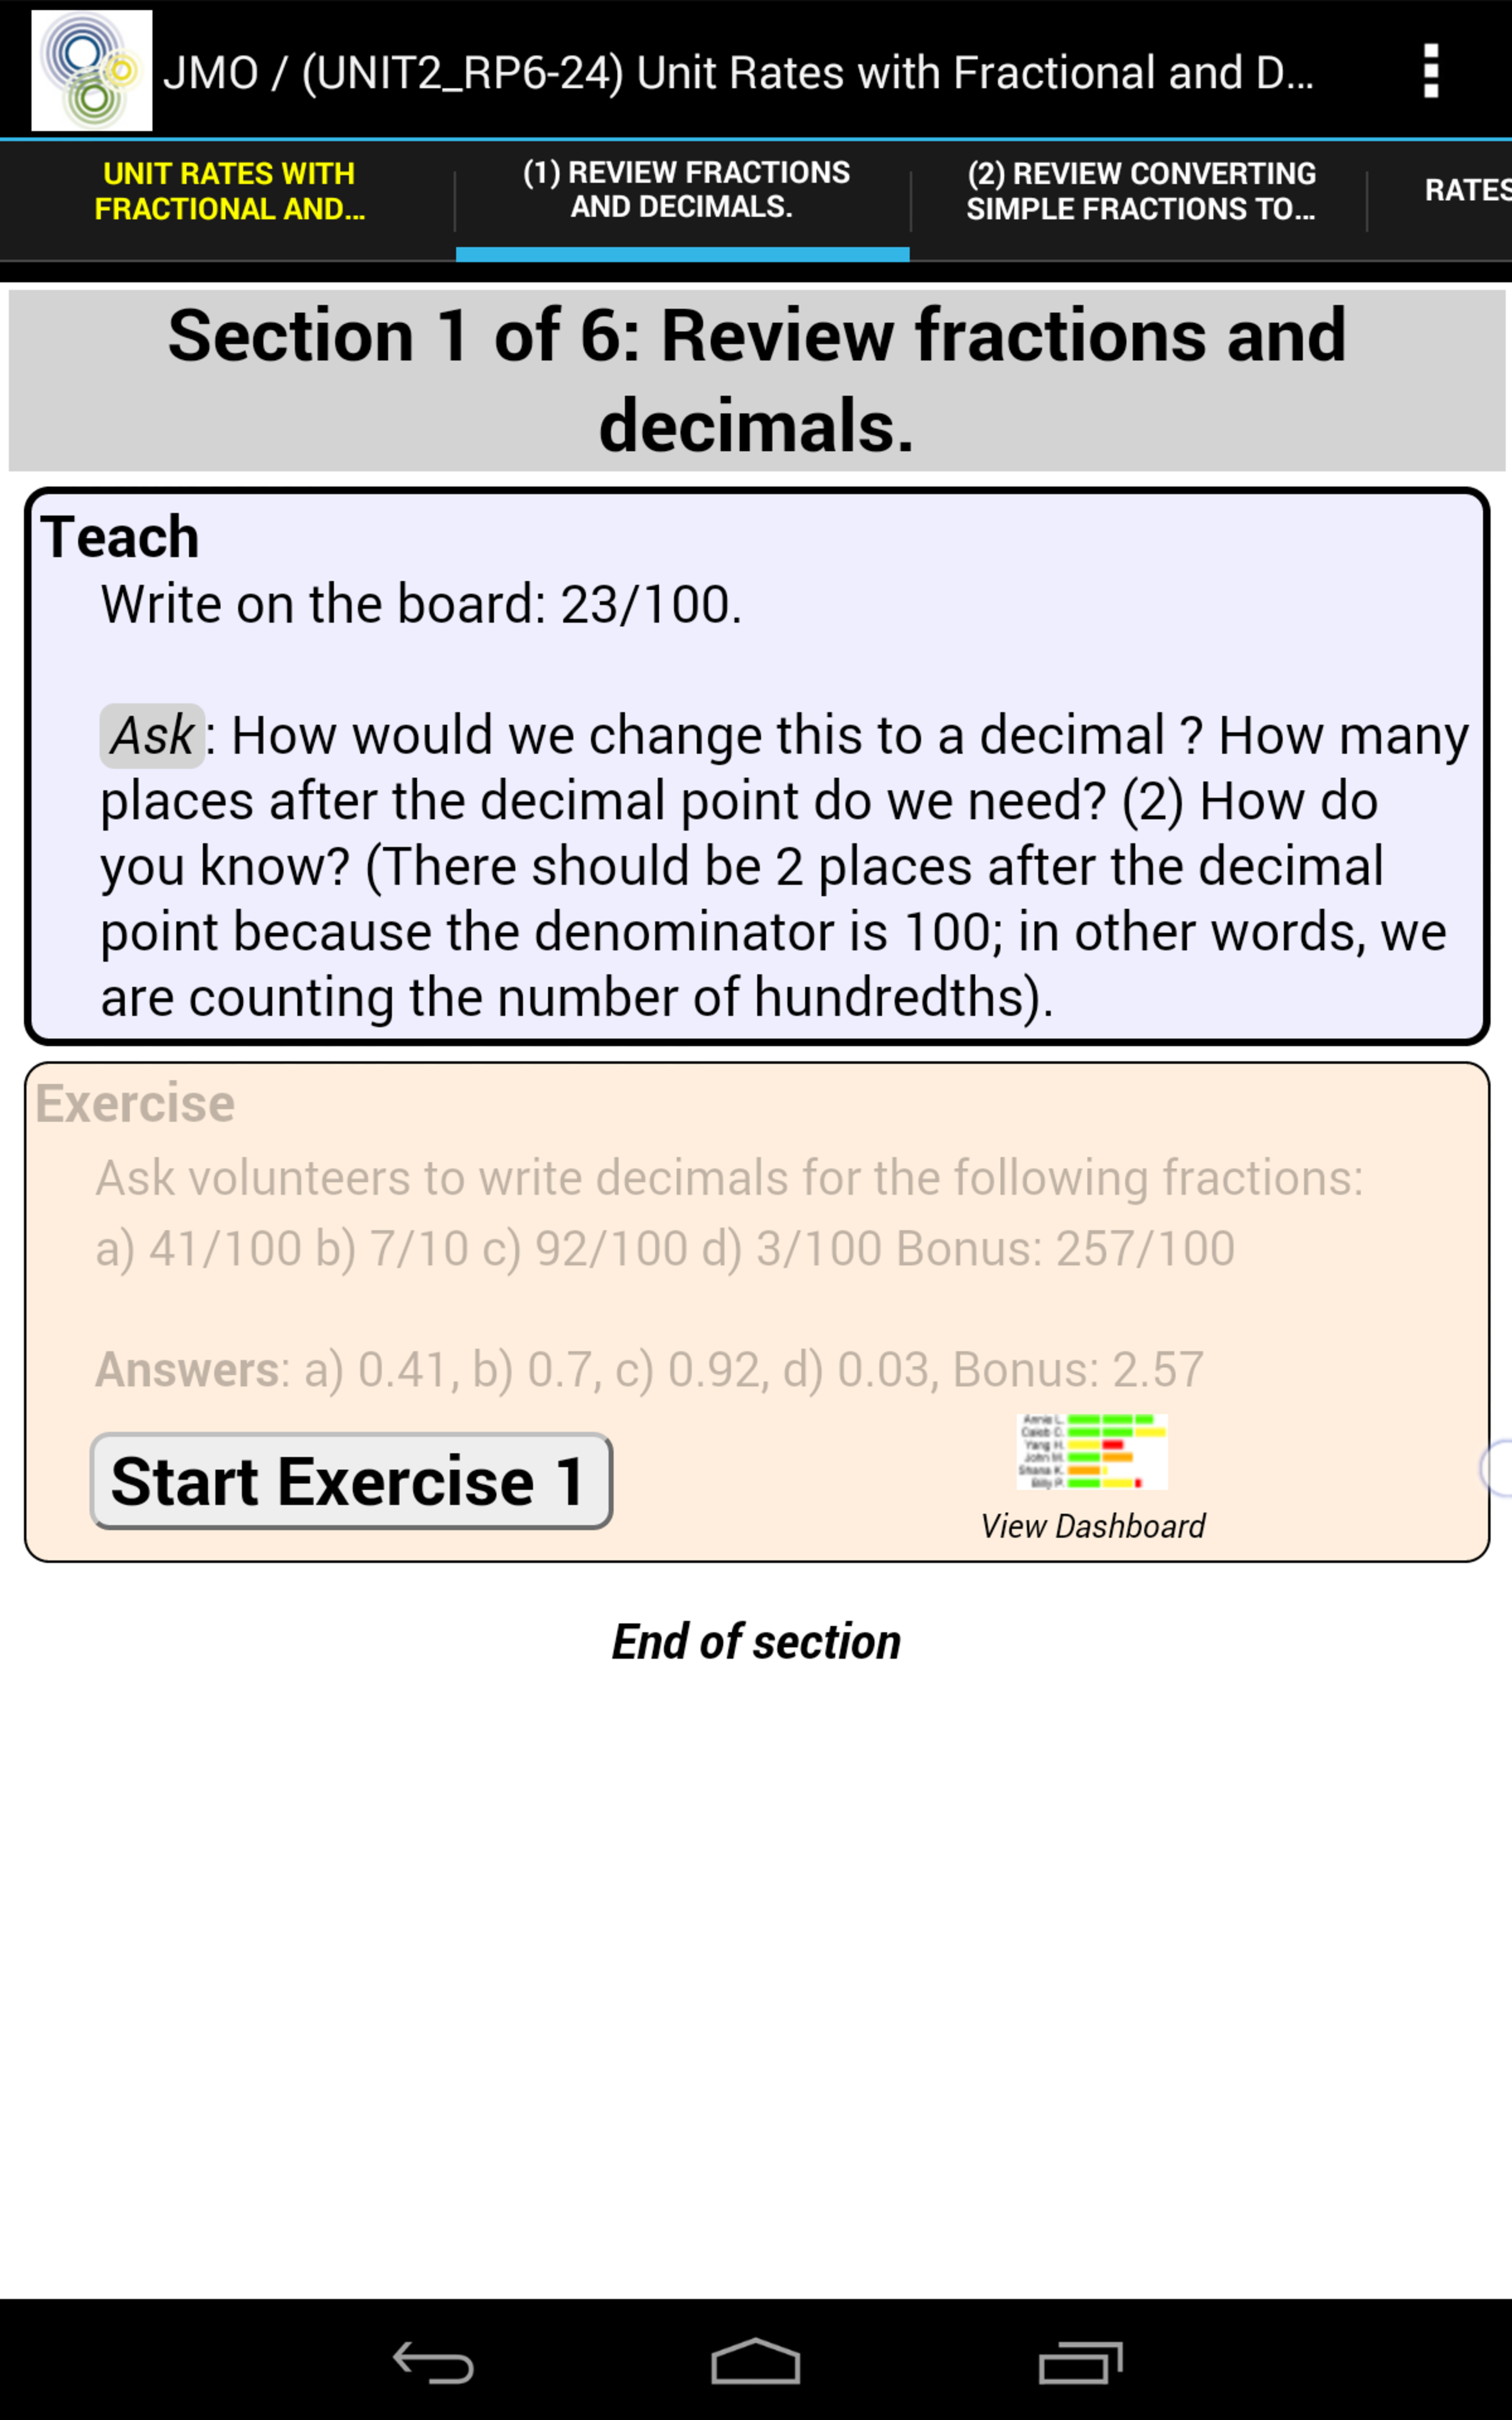
\includegraphics[width=40mm]{images/TeacherEX.pdf}} \hspace{1em}%
%\subfigure[]{\label{fig:TeacherDashboard}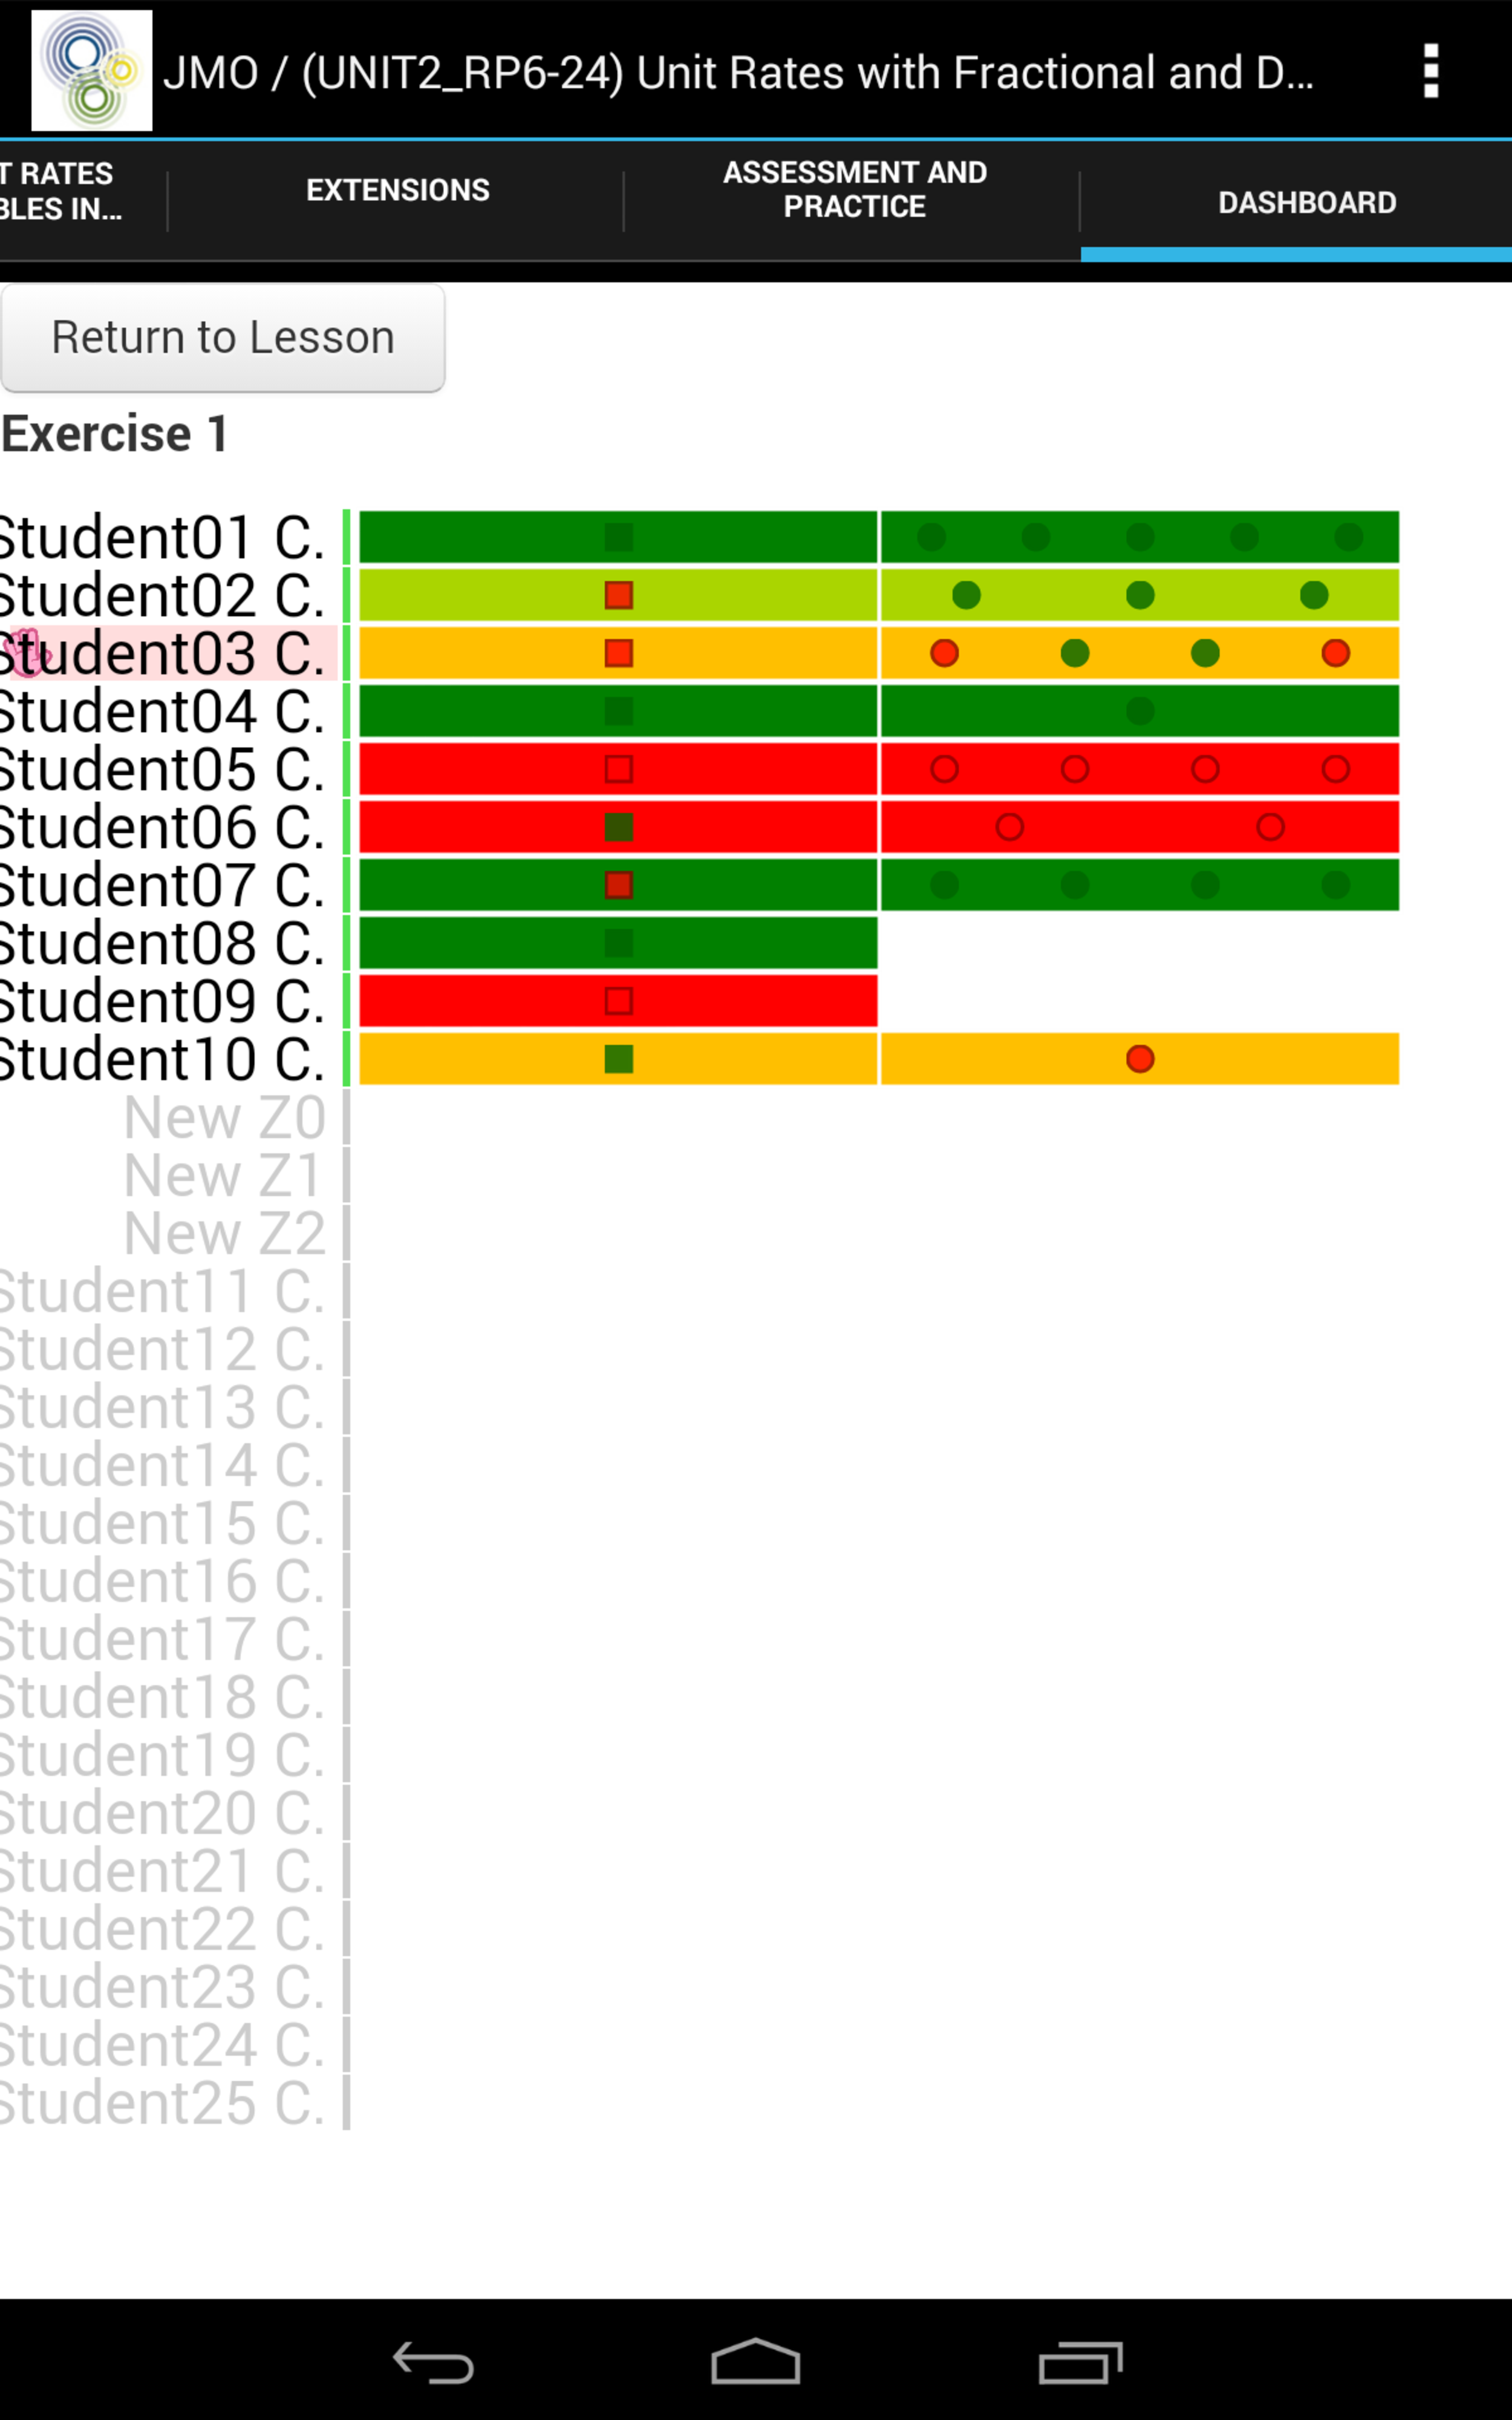
\includegraphics[width=40mm]{images/TeacherDashboard.pdf}} \hspace{1em}%
%\subfigure[]{\label{fig:StudentProblemSolving}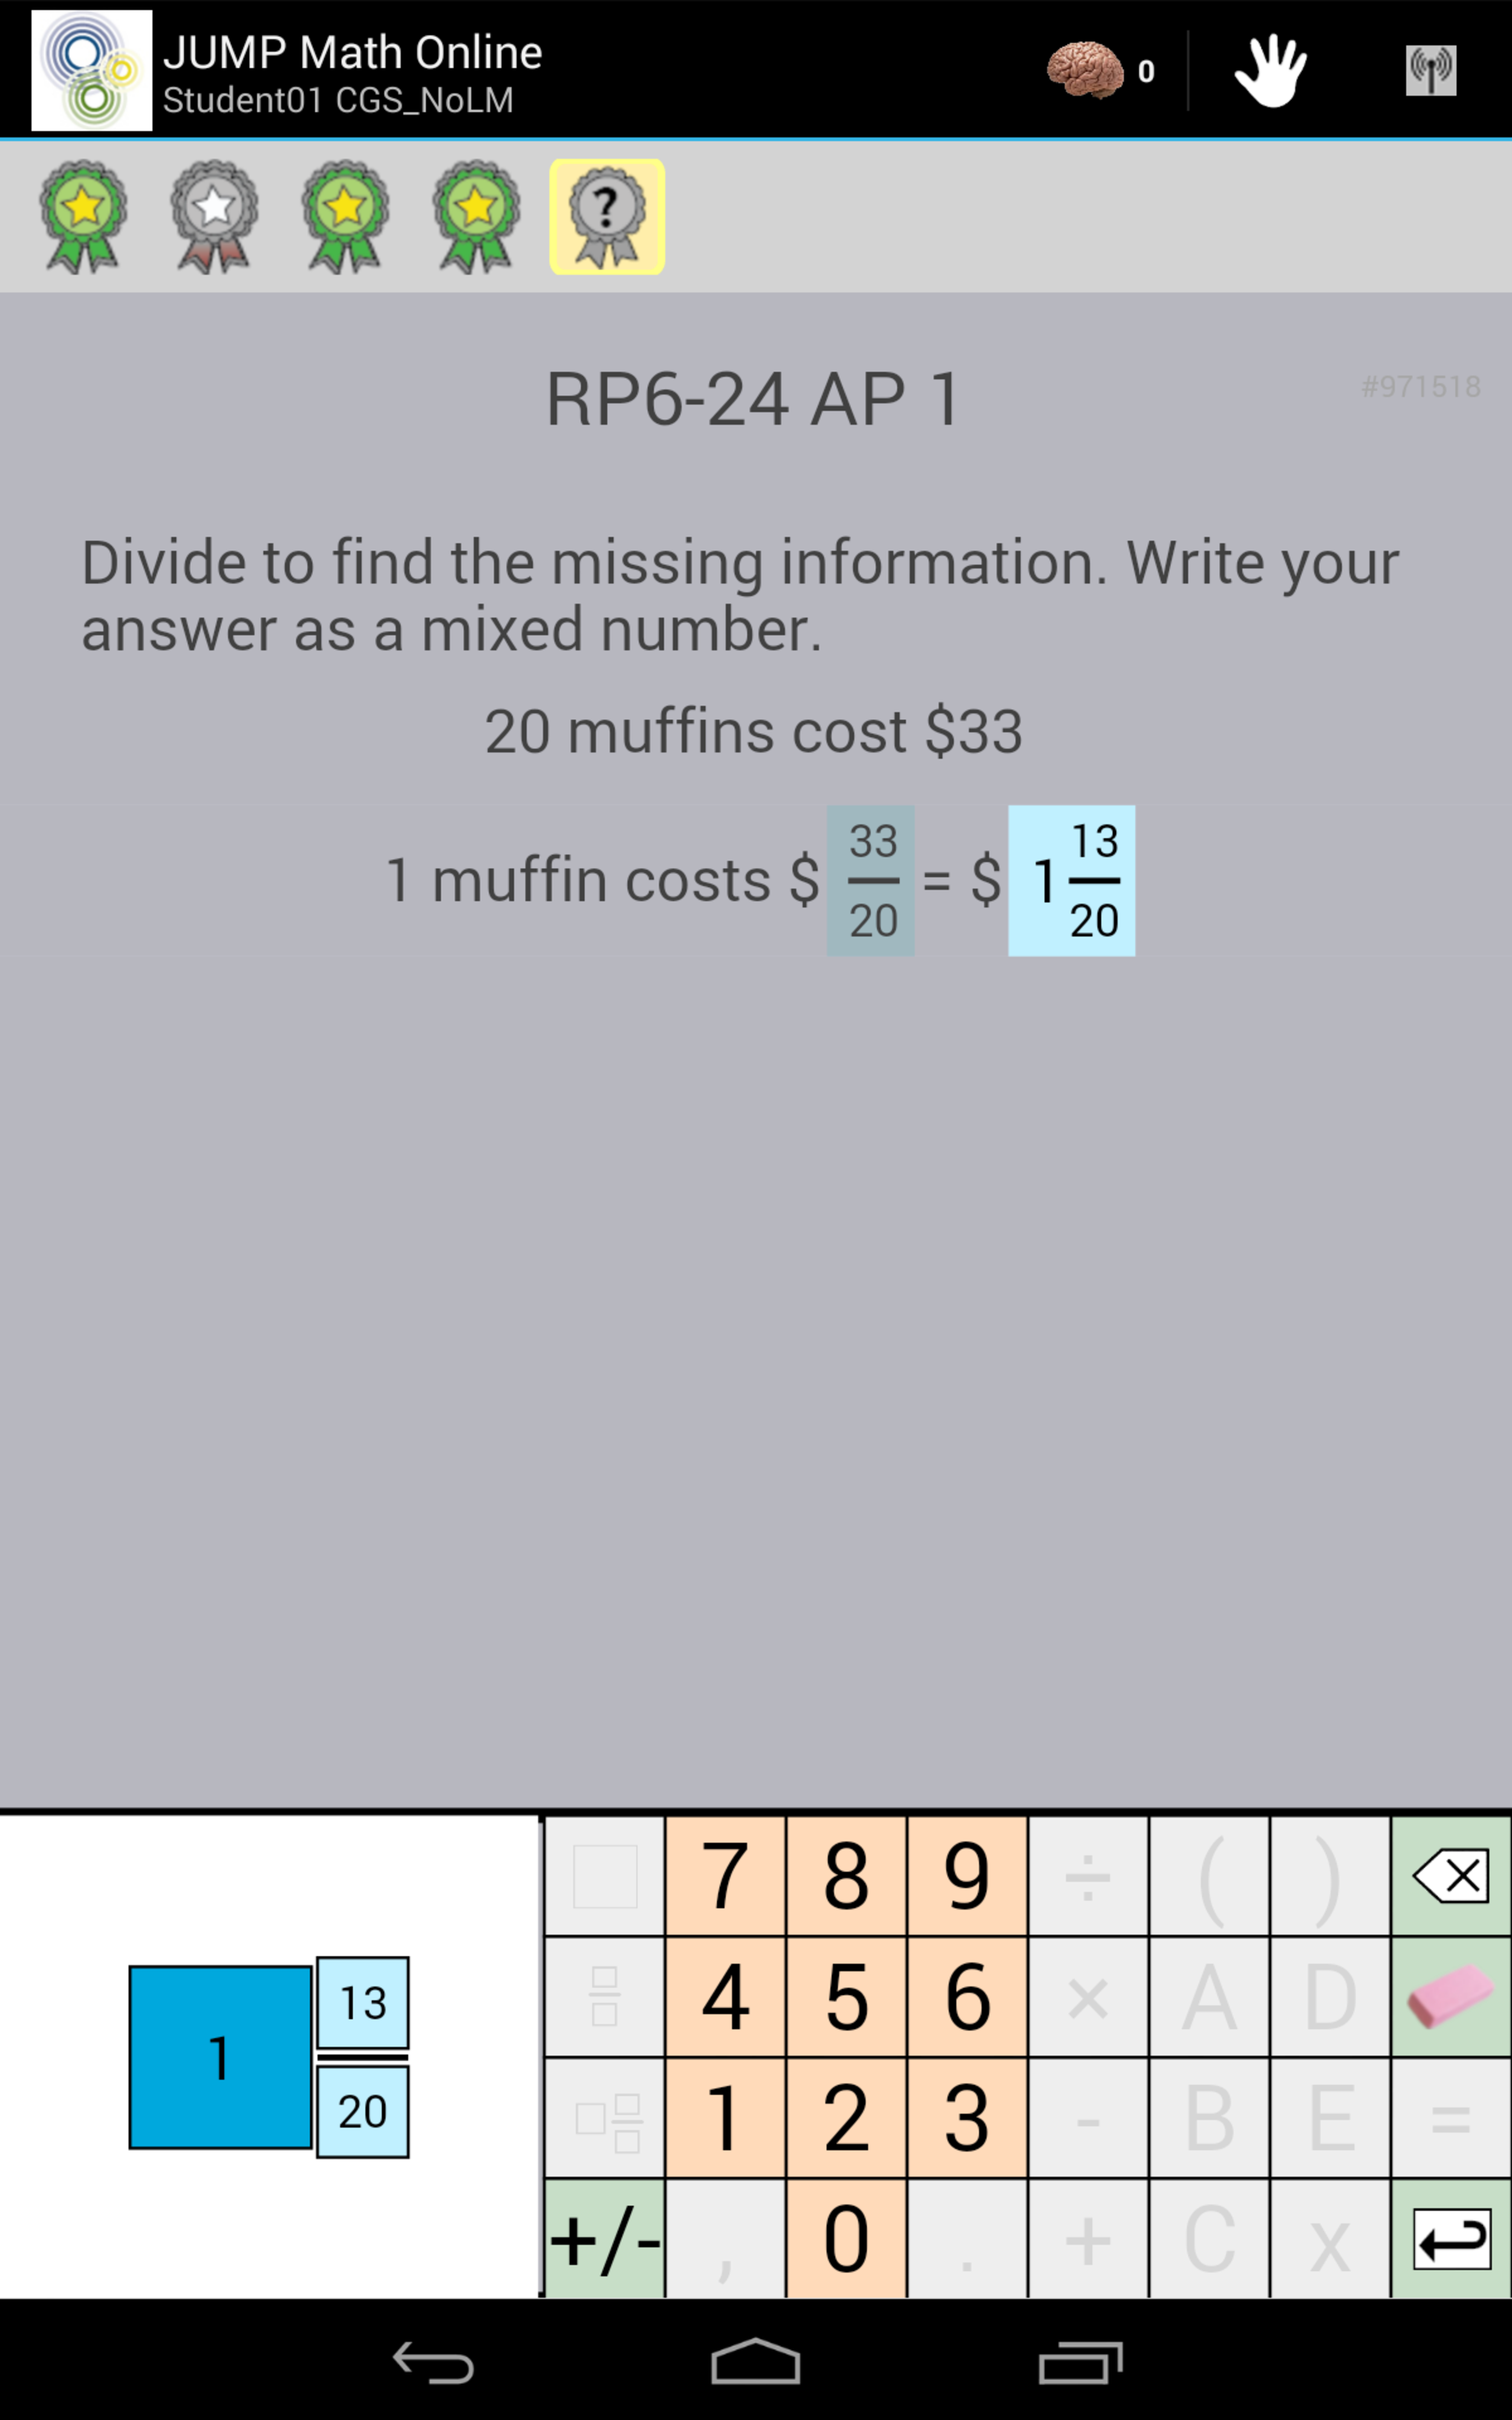
\includegraphics[width=40mm]{images/Student.pdf}}
%\caption{
%Screenshots of the Teacher and Student software. Figure (a) shows the teacher lesson view. Figure (b) shows a prompt for the teacher to ``Start Exercise 1'' on all student tablets. Figure (c) shows the teacher Dashboard that displays student problem-solving progress. Figure (d) shows the student problem-solving interface, with a calculator input interface at the bottom of the screen and badges at the top that indicate problem correctness. }
%\label{fig:Spreadsheet}
%\end{figure*}


% Balancing columns in a ref list is a bit of a pain because you
% either use a hack like flushend or balance, or manually insert
% a column break.  http://www.tex.ac.uk/cgi-bin/texfaq2html?label=balance
% multicols doesn't work because we're already in two-column mode,
% and flushend isn't awesome, so I choose balance.  See this
% for more info: http://cs.brown.edu/system/software/latex/doc/balance.pdf
%
% Note that in a perfect world balance wants to be in the first
% column of the last page.
%
% If balance doesn't work for you, you can remove that and
% hard-code a column break into the bbl file right before you
% submit:
%
% http://stackoverflow.com/questions/2149854/how-to-manually-equalize-columns-
% in-an-ieee-paper-if-using-bibtex
%
% Or, just remove \balance and give up on balancing the last page.
%
%\balance{}


% REFERENCES FORMAT
% References must be the same font size as other body text.
\bibliographystyle{SIGCHI-Reference-Format}
\bibliography{references}

\end{document}

%%% Local Variables:
%%% mode: latex
%%% TeX-master: t
%%% End:
